\section{Колебания физического маятника}

\introProblems

\begin{ex} %Сив599
В какой точке следует подвесить однородный стержень длины  $l$, чтобы частота его колебаний, как физического маятника, была максимальна? Чему равна эта частота?
\begin{ans}
$x = l/(2\sqrt{3})$, $\omega^2 = g\sqrt{3} / l$.
\end{ans}
\end{ex}	

\begin{ex} %Сив602
На горизонтальной плоскости находится цилиндр с моментом инерции $I$ (относительно продольной геометрической оси), массой $m$ и радиусом $r$. К оси цилиндра прикреплены две одинаковые горизонтально расположенные спиральные пружины, другие концы которых закреплены в стене (рис. \ref{rollOscil}, вид сверху). Коэффициент жесткости каждой пружины равен $k$; пружины могут работать как на растяжение, так и на сжатие. Найти период малых колебаний цилиндра, которые возникнут, если вывести его из положения равновесия и дать возможность кататься без скольжения по горизонтальной плоскости.
\begin{ans}
$T =  \pi\sqrt{3m/k}$.
\end{ans}
\end{ex}	

\begin{figure}[h]
\centering
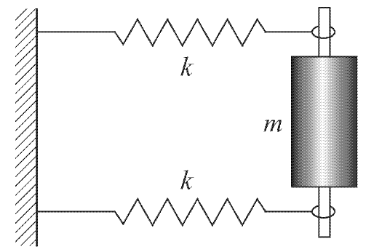
\includegraphics[width=0.4\textwidth]{rollOscil.png}
\caption{}
\label{rollOscil}
\end{figure}

\begin{ex} %Сив607
Найти период малых колебаний физического маятника массы $m$, к центру масс $C$ которого прикреплена горизонтальная спиральная пружина с коэффициентом жесткости $k$. Другой конец пружины закреплен в неподвижной стенке (рис. \ref{physPend}). Момент инерции маятника относительно точки подвеса равен $I$, расстояние между точкой подвеса и центром масс маятника равно $a$. В положении равновесия пружина не деформирована.
\begin{ans}
$T = 2 \pi \sqrt{I/(mga + ka^2)}$.
\end{ans}
\end{ex}	

\begin{figure}[h]
\centering
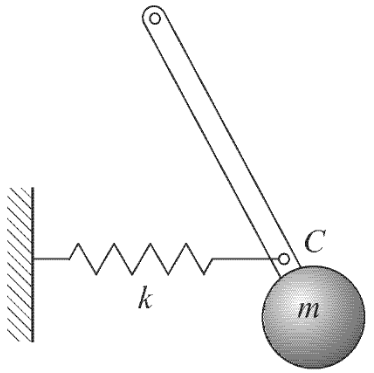
\includegraphics[width=0.3\textwidth]{physPend.png}
\caption{}
\label{physPend}
\end{figure}

\begin{ex} %Сив608
Колебательная система состоит из однородного стержня длины $l$ и массы $m$, который может вращаться вокруг горизонтальной оси $O$, проходящей через его конец и перпендикулярной к продольной оси стержня (рис. \ref{springRodOsc}). Другой конец стержня подвешен на пружине с коэффициентом жесткости $k$. Расстояние между серединой стержня и осью вращения $CO = a$. Момент инерции стержня относительно оси $O$ равен $I$. Найти удлинение пружины $x_0$ (по сравнению с ее длиной в недеформированном состоянии) в положении равновесия, если в этом $O$ положении стержень горизонтален. Определить также период малых колебаний стержня около положения равновесия.
\begin{ans}
$x_0 = mga/kl$, $T = 2 \pi \sqrt{I/kl^2}$.
\end{ans}
\end{ex}	

\begin{figure}[h]
\centering
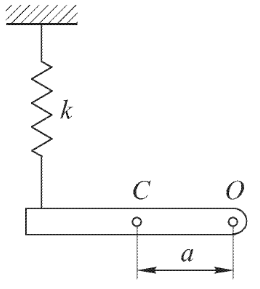
\includegraphics[width=0.3\textwidth]{springRodOsc.png}
\caption{}
\label{springRodOsc}
\end{figure}

\qualProblems

\begin{ex}
Мальчик качается на качелях сидя. Изменится ли период колебания, если он будет качаться стоя? Если подсядет еще один мальчик.
\end{ex}	

\begin{ex}
Лифт вначале движется равноускоренно, замет равномерно и равнозамедленно. Как изменится период колебания математического (нитяного) маятника в лифте?
\end{ex}	

\begin{ex}
Часы-ходики установлены в вагоне электрички. Отстанут или забегут часы, когда электричка, вышедшая из Екатеринбурга, прибудет, например, в Нижний Тагил, сделав примерно тридцать остановок на промежуточных станциях.
\end{ex}	

\begin{ex}
Почему так ужасно скрипит мел, если мы неправильно держим его, когда пишем на доске? Как влияет при этом положение мела относительно доски и чем определяется частота издаваемого им звука?
\end{ex}	

\begin{ex}
Два шара одинаковых размеров подвешены на одинаковых нитях. Один шар сделан из свинца, а другой – из алюминия. Шары покрыты краской так, что внешне они неразличимы. Как, наблюдая за колебаниями шаров, найти свинцовый шар?
\end{ex}	

\begin{ex}
Как будет изменяться период колебаний ведерка с водой, если из него вода будет постепенно вытекать через небольшое отверстие в днище?
\end{ex}	

\simpleProblems

\begin{ex} %Сив592
Сплошной однородный диск с радиусом $r = 10$ см колеблется около оси, перпендикулярной к плоскости диска и проходящей через край диска. Какой длины $l$ должен быть математический маятник, имеющий тот же период колебаний, что и диск?
\begin{ans}
$l = 15$ см.
\end{ans}
\end{ex}	

\begin{ex} %Сив619
На горизонтальной пружине укреплено тело массы $M = 10$ кг, лежащее на гладком столе, по которому оно может скользить без трения (рис. \ref{shootOsc}). В это тело попадает и застревает в нем пуля массы $m = 10$ г, летящая с горизонтальной скоростью $v = 500$ м/с, направленной вдоль оси пружины. Тело вместе с застрявшей в нем пулей отклоняется от положения равновесия и начинает колебаться относительно него с амплитудой $A = 10$ см. Найти период колебаний тела.
\begin{ans}
$T = 2 \pi (M+m) / mv = 1,26$ с.
\end{ans}
\end{ex}	

\begin{figure}[h]
\centering
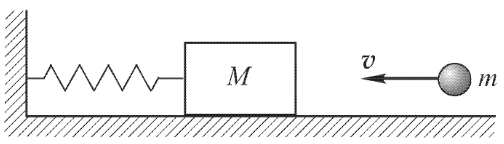
\includegraphics[width=0.5\textwidth]{shootOsc.png}
\caption{}
\label{shootOsc}
\end{figure}

\begin{ex} %Сив598
Маятник метронома представляет собой груз $M$, качающийся около оси $O$, с прикрепленной к нему спицей, по которой может перемещаться малый груз m (рис. \ref{metronom}). Как зависит период колебаний маятника от координаты $x$ грузика? Массу $m$ считать точечной. Момент инерции маятника метронома относительно оси $O$ равен $I$.
\begin{ans}
$T = 2 \pi \sqrt{(I+mx^2)/(Ma - mx)}$.
\end{ans}
\end{ex}	

\begin{figure}[h]
\centering
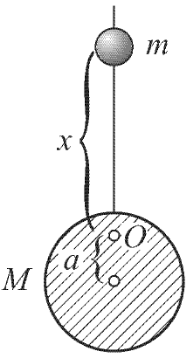
\includegraphics[width=0.2\textwidth]{metronom.png}
\caption{}
\label{metronom}
\end{figure}

\begin{ex} %Сив605
Шарик массы $m$ подвешен на двух последовательно соединенных пружинках с коэффициентами жесткости $k_1$ и $k_2$. Определить период его вертикальных колебаний.
\begin{ans}
$T = 2 \pi \sqrt{m(1/k_1 + 1/k_2)}$.
\end{ans}
\end{ex}	

\begin{ex} %Сив610
Два незакрепленных шарика с массами $m_1$ и $m_2$ соединены друг с другом спиральной пружинкой с коэффициентом жесткости $k$. Определить период колебаний шариков относительно центра масс системы, которые возникнут при растяжении пружинки.
\begin{ans}
$T = 2 \pi \sqrt{m_1m_2/(m_1 + m_2)k}$.
\end{ans}
\end{ex}	

\complexProblems

\begin{ex} %Сив587
Однородная палочка подвешена за оба конца на двух одинаковых нитях длины $L$. В состоянии равновесия обе нити параллельны. Найти период $T$ малых колебаний, возникающих после некоторого поворота палочки вокруг вертикальной оси, проходящей через середину палочки.
\begin{ans}
$T = 2 \pi \sqrt{L/3g}$.
\end{ans}
\end{ex}	

\begin{figure}[h]
\centering
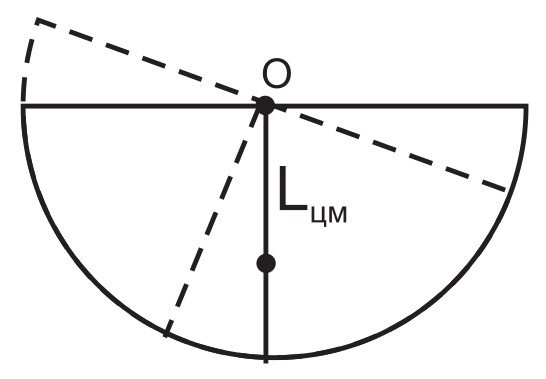
\includegraphics[width=0.3\textwidth]{halfRingOscill.png}
\caption{}
\label{halfRingOscill}
\end{figure}

\begin{ex}
Из тонкой проволоки сделали замкнутую фигуру, изображенную на рисунке \ref{halfRingOscill}. Радиус окружности равен $R$. Где находится
центр тяжести этой фигуры? Чему равен период малых колебаний относительно точки О?
\begin{ans}
$L_C = 2R/(2 + \pi), T = 2 \pi (2 + 3\pi)/(6g)$.
\end{ans}
\end{ex}	

\clearpage